\input{praeambel_gesina.tex}

%Folgende Pakete zusätzlich im Header einfügen:
\usepackage{tikz,pgf}
\usetikzlibrary{arrows}
\usetikzlibrary{matrix}
\usetikzlibrary{decorations.pathmorphing}

\begin{document}
\section*{Bild mit label 2.1.3.im1}
	\centering 
	\LARGE
	\[
		\begin{pmatrix}
			\hspace{0.15cm}
			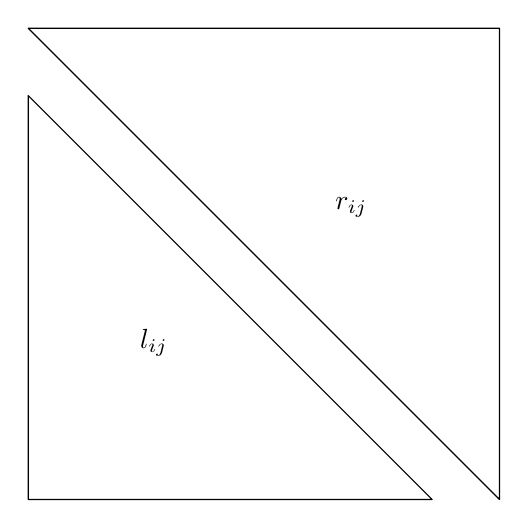
\begin{tikzpicture}[scale=5.7,line cap=round,line join=round,>=triangle 45,x=1.0cm,y=1.0cm]
				\draw[color=black] (0,0) -- (0,0.9) -- (0.9,0) -- cycle;
				\draw[color=black] (0.28,0.35) node {$l_{ij}$};
				\draw[color=black] (1.05,0) -- (1.05,1.05) -- (0,1.05) -- cycle;
				\draw[color=black] (0.72,0.65) node {$r_{ij}$};
			\end{tikzpicture}
			\hspace{0.15cm}
		\end{pmatrix}\hspace{0.5cm}
		\begin{pmatrix}
			\hspace{0.15cm}
				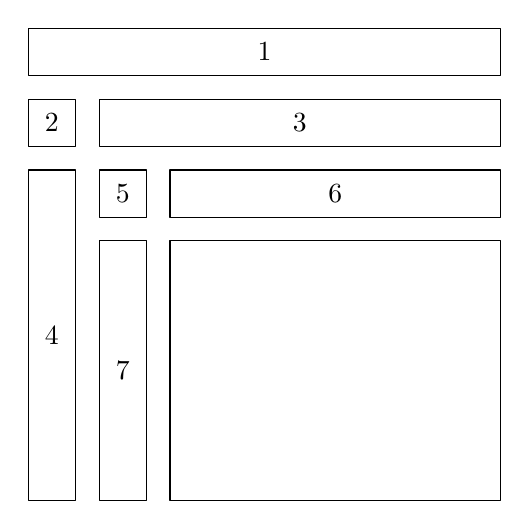
\begin{tikzpicture}[scale=3,line cap=round,line join=round,>=triangle 45,x=1.0cm,y=1.0cm]
					\draw (0,1.8) rectangle (2,2);
					\draw (1,1.9) node {1};
					
					\draw (0.2,1.5) rectangle (0,1.7);
					\draw (0.1,1.6) node {2};
					
					\draw (0.3,1.5) rectangle (2,1.7);
					\draw (1.15,1.6) node {3};
					
					\draw (0,0) rectangle (0.2,1.4);
					\draw (0.1,0.7) node {4};
					
					\draw (0.3,1.2) rectangle (0.5,1.4);
					\draw (0.4,1.3) node {5};
					
					\draw (0.6,1.2) rectangle (2,1.4);
					\draw (1.3,1.3) node {6};
					
					\draw (0.3, 0) rectangle (0.5,1.1);
					\draw (0.4,0.55) node {7};
					
					\draw (0.6,0) rectangle (2,1.1);
				\end{tikzpicture}
			\hspace{0.15cm}
		\end{pmatrix}
	\]
\section*{Grafiken zum Beweis von 2.1.13}
	\[
		\begin{pmatrix}
			\begin{tikzpicture}[scale=4,line cap=round,line join=round,>=triangle 45,x=1.0cm,y=1.0cm]
				\draw (0,1.8) rectangle (2,2);
				\draw (1,1.9) node {1};
				
				\draw (0,0) rectangle (0.2,1.7);
				\draw (0.1,0.85) node {2};
				
				\draw (0.3,1.5) rectangle (2,1.7);
				\draw (1.15,1.6) node {3};
				
				\draw (0.3,0) rectangle (0.5,1.4);
				\draw (0.4,0.7) node {4};
				
				\draw (0.6,1.2) rectangle (2,1.4);
				\draw (1.3,1.3) node {5};
				
			\end{tikzpicture}
		\end{pmatrix}
	\]
	
	%2. Grafik
	\[
		\begin{pmatrix}
			\begin{tikzpicture}[scale=4,line cap=round,line join=round,>=triangle 45,x=1.0cm,y=1.0cm]
				\draw (0,1.8) -- (0.2,1.8) -- (0.2,2);
				\draw (0.1,1.9) node {1};
				
				\draw (0,1.5) -- (0.5,1.5) -- (0.5,2);
				\draw (0.35,1.65) node {2};
				
				\draw (0,1.2) -- (0.8,1.2) -- (0.8,2);
				\draw (0.65,1.35) node {3};
				
				\draw[color = white] (2,2) -- (2,0);
			\end{tikzpicture}
		\end{pmatrix}
	\]
	%Zeilenweise
	\[
		\begin{pmatrix}
			\begin{tikzpicture}[scale=4,line cap=round,line join=round,>=triangle 45,x=1.0cm,y=1.0cm]
				\draw (0,1.8) rectangle (2,2);
				\draw (1,1.9) node {1};
				
				\draw (0,1.5) rectangle (0.2,1.7);
				\draw (0.1,1.6) node {2};
				
				\draw (0.3,1.5) rectangle (2,1.7);
				\draw (1.15,1.6) node {3};
				
				\draw (0,1.2) rectangle (0.5,1.4);
				\draw (0.25,1.3) node {4};
				
				\draw (0.6,1.2) rectangle (2,1.4);
				\draw (1.3,1.3) node {5};
				
				\draw (0,0.9) rectangle (0.8,1.1);
				\draw (0.4,1) node {6};
				
				\draw (0.9,0.9) rectangle (2,1.1);
				\draw (1.45,1) node {7};
				
				\draw[color=white] (0,0) -- (2,0);
			\end{tikzpicture}
		\end{pmatrix}
	\]
	
\section*{imagemissing\{Diagramm zur Rückwärtsanalyse\}}
	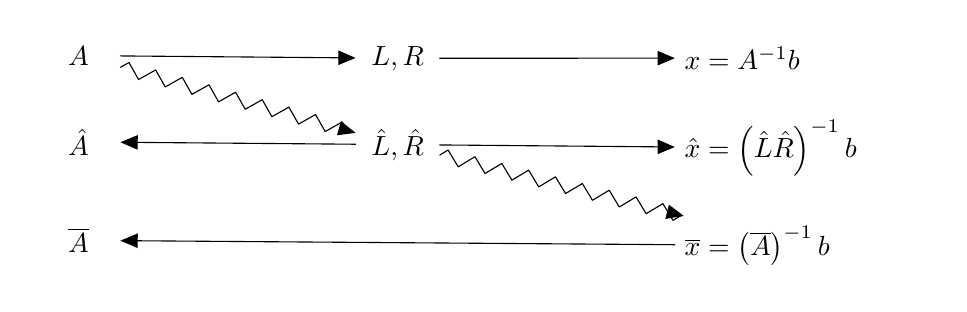
\begin{tikzpicture}[scale=1,line cap=round,line join=round,>=triangle 45,x=1.0cm,y=1.0cm]
		\matrix (m) [matrix of math nodes,row sep=0.4cm,column sep=3cm,minimum width=3em]
		{
			A &L,R & \parbox{3cm}{$x=A^{-1}b$}\\
			\hat{A} &\hat{L},\hat{R} &\parbox{3cm}{$ \hat{x}=\left(\hat{L}\hat{R}\right)^{-1}b$}\\
			\overline{A}&&\parbox{3cm}{$\overline{x}=\left(\overline{A}\right)^{-1}b$}\\
		};
		\path
		(m-1-1) edge [->](m-1-2)
		        edge [->,decorate,decoration=zigzag](m-2-2)
		(m-1-2) edge [->](m-1-3)
		(m-2-1) edge [<-] (m-2-2)
		(m-2-2) edge [->] (m-2-3)
				edge [->,decorate,decoration=zigzag](m-3-3)
		(m-3-1) edge [<-] (m-3-3);
	\end{tikzpicture}

\section*{Grafik in 4.3.2}
	\begin{tikzpicture}[rotate=14,line cap=round,line join=round,>=triangle 45,x=1.0cm,y=1.0cm]
		\clip(1.8,-3.2) rectangle (12,3);
		\draw [shift={(6,0)}] (0,0) -- (90:0.6) arc (90:180:0.6) -- cycle;
		\draw (2,2)-- (10,2);
		\draw (10,2)-- (10,-2);
		\draw (10,-2)-- (2,-2);
		\draw (2,-2)-- (2,2);
		\draw (4,0)-- (6,0);
		\draw (6,0)-- (6,2.46);
		\fill (5.75,0.25) circle (0.02);
		\draw (8,-2.5) node[anchor= west] {$Ax\text{ f\"ur }b\in\mathbb{R}^3$};
		\draw (10,-1)-- (10.68,-0.88);
		\draw (10.84,-0.36) node [anchor=north west] {$R(A)$};
		\draw [->] (8,-2.6) -- (6.72,-2.14);
		\fill  (4,0) circle (1.5pt);
		\draw (3.86,-0.18) node {0};
		\fill  (6,0) circle (1.5pt);
		\draw(6.22,0.26) node {$A\overline{x}$};
		\fill  (6,2.46) circle (1.5pt);
		\draw (6.16,2.72) node {$b$};
	\end{tikzpicture}
\section*{Grafik in 4.4.b}
	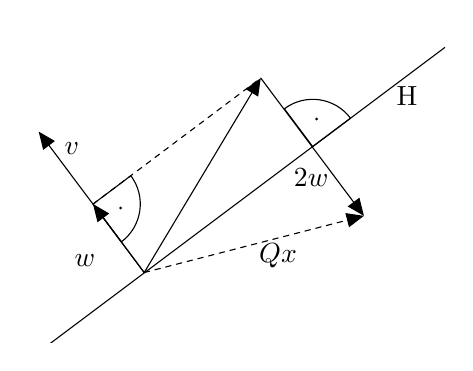
\begin{tikzpicture}[line cap=round,line join=round,>=triangle 45,x=1.0cm,y=1.0cm]
		\clip(0.7,1) rectangle (6,5);
		\draw [shift={(4.32,3.49)}] (0,0) -- (36.87:0.6) arc 	(36.87:126.87:0.6) -- cycle;
		\draw [shift={(1.53,2.76)}] (0,0) -- (-53.13:0.6) arc (-53.13:36.87:0.6) -- cycle;
		\draw [domain=0.7:6] plot(\x,{(--1--3*\x)/4});
		\draw (5.26,4.38) node[anchor=north west] {$$H$$};
		\draw [->] (2.18,1.89) -- (0.84,3.68);
		\draw [->] (2.18,1.89) -- (3.66,4.36);
		\draw [->] (2.18,1.89) -- (1.53,2.76);
		\draw [->,dash pattern=on 2pt off 2pt] (2.18,1.89) -- (4.97,2.61);
		\draw [->] (3.66,4.36) -- (4.97,2.61);
		\fill(4.37,3.84) circle (0.02);
		\draw [dash pattern=on 2pt off 2pt] (1.53,2.76)-- (3.66,4.36);
		\fill(1.88,2.71) circle (0.02);
	
		\draw (1.26,3.46) node {$v$};
		\draw (1.68,2.24) node[anchor=north east] {$w$};
		\draw (3.88,2.1) node {$Qx$};
		\draw (4.3,3.1) node {$2w$};
	\end{tikzpicture}

\end{document}
